
\chapter{Modbus Secure}
\label{secure}

Il protocollo Modbus Secure utilizza gli stessi frame del protocollo TCP
standard incapsulati tramite TLS.
Il protocollo TLS fornisce un sistema di autenticazione tramite certificati x.509v3. 
La normativa richiede
TLS con versione 1.2 o superiore (attualmente siamo alla versione 1.3),
il client supporta entrambe le versioni (1.2 e 1.3). 
L'utilizzo dei certificati richiede la creazione di un certificato e di una chiave
privata per il server, così come per ogni client che si collegherà al gateway. 
Si riporta di seguito una schema per chiarire i
ruoli dei certificati sia lato server che client:

\begin{figure}[H]
  \centering
  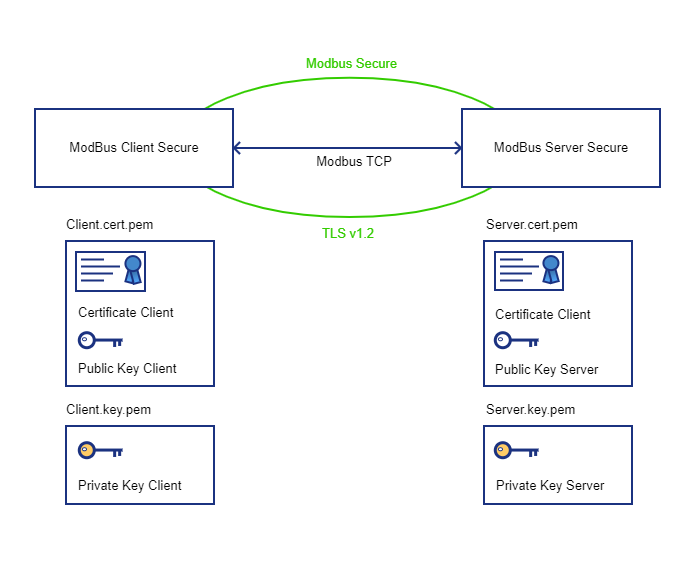
\includegraphics[width=0.8\textwidth]{../Img/schemamodbussecure.png}
  \caption{Schema certificati Modbus Secure}
\end{figure}

La normativa richiede di aggiungere al certificato x.509v3 alcune estensioni tra cui un OID (Object
Identifier standardized by the International Telecomunications Union) per definire il ruolo del client al
momento dell'autenticazione. La specifica prevede infatti che tutti i client possano utilizzare funzioni di
lettura ma solo i client con il ruolo di "operator" possano utilizzare funzioni di scrittura (di coils o holding
registers).

\newpage
\section{Specifiche normativa}

Si riportano di seguito le specifiche principali della normativa (MB-TCP\_Security-v21\_2018-07-24):

\begin{itemize}
    \item Il protocollo utilizzato deve essere $\ge$ TLS 1.2
    \item Cipher suite: RSA per key exchange
    \item Cipher suite: AES128 per cifratura dei pacchetti
    \item Cipher suite: SHA256SUM per il controllo di integrità dei messaggi
    \item Default cipher: TLS\_RSA\_WITH\_AES\_128\_CBC\_SHA256
\end{itemize}

\section{Estensioni X509v3}

Si riporta di seguito il contenuto delle estensioni che richiede la normativa 
da aggiungere ad un certificato X509v3 standard:

\begin{verbatim}
X509v3 extensions:
  X509v3 Subject Key Identifier:
      38:A4:CC:19:6D:6D:E2:AA:7C:82:75:44:A0:59:39:81:47:D3:13:F0
  X509v3 Authority Key Identifier:
      keyid:38:A4:CC:19:6D:6D:E2:AA:7C:82:75:44:A0:59:39:81:47:D3:13:F0

  X509v3 Basic Constraints:
      CA:FALSE
  X509v3 Key Usage: critical
      Digital Signature, Non Repudiation, Key Encipherment
  1.3.6.1.4.1.50316.802.1:
      ..Operator
  X509v3 Subject Alternative Name:
      IP Address:192.168.1.10
\end{verbatim}

\newpage
\section{Generazione dei certificati}

Gli step per generare i certificati con openssl 
sono i seguenti (sono gestite le righe multiple per cui si 
possono copiare e incollare i comandi direttamente sulla shell):
\\\\
Generare certificato e chiave privata per il server (modificando l'ip con l'indirizzo corretto del server):

\begin{verbatim}
# Server
  openssl req -x509 -newkey rsa:4096 -sha256 -days 360 \
  -keyout server.key.pem -out server.cert.pem \
  -nodes -subj "/C=IT/ST=Italy/L=Rovereto/O=ModBusServer/OU=ModBusServer/CN=ModbusSecurityServer" \
  -addext "keyUsage=critical,digitalSignature,nonRepudiation,keyEncipherment" \
  -addext "subjectAltName=IP:192.168.1.20"
\end{verbatim}

Generare uno o più certificati/chiavi private per i client che 
vorranno collegarsi al server (si riportano tre esempi di seguito, anche in questo caso va aggiornato l'ip):

\begin{verbatim}
# Client 1:
  openssl req -x509 -newkey rsa:4096 -sha256 -days 360 \
  -keyout client1.key.pem -out client1.cert.pem -nodes \
  -subj "/C=IT/ST=Italy/L=Rovereto/O=ModBusClient/OU=ModBusClient/CN=ModbusSecurityClient" \
  -addext "keyUsage=critical,digitalSignature,nonRepudiation,keyEncipherment" \
  -addext "1.3.6.1.4.1.50316.802.1=ASN1:UTF8String:Operator" \
  -addext "subjectAltName=IP:192.168.1.10"
\end{verbatim}

Su windows molto spesso l'abbinata certificato+chiave private viene unita in un unico file protetto da password (.pfx),
Per unire certificato e chiave in un file pfx usare il comando seguente:

\begin{verbatim}
  openssl pkcs12 -export -out client1.pfx -inkey client1.key.pem -in client1.cert.pem
\end{verbatim}

Per aprire un certificato visualizzare il contenuto si può usare il comando:

\begin{verbatim}
  openssl x509 -in client1.cert.pem -text
\end{verbatim}
